\documentclass[a4paper,twoside]{article}
\usepackage{epsfig}
\usepackage{subfigure}
\usepackage{calc}
\usepackage{amssymb}
\usepackage{amstext}
\usepackage{amsmath}
\usepackage{amsthm}
\usepackage{multicol}
\usepackage{pslatex}
\usepackage{apalike}
\usepackage{SCITEPRESS}
\usepackage[small]{caption}
\usepackage{hyperref}

\subfigtopskip=0pt
\subfigcapskip=0pt
\subfigbottomskip=0pt

\hyphenation{ge-ne-ral-ly}
\hyphenation{BadVoltage}
\hyphenation{CoverOpenAlert}
\hyphenation{con-sis-ting}
\hyphenation{ca-pa-ci-ty}
\hyphenation{exam-ple}
\hyphenation{prio-ri-ty}
\hyphenation{re-le-vant}
\hyphenation{pro-cessing}
\hyphenation{ge-ne-ra-ted}
\hyphenation{me-mo-ry}
\hyphenation{ta-king}
\hyphenation{con-si-de-red}
\hyphenation{cons-train}
\hyphenation{ins-tan-ce}
\hyphenation{ins-tan-ces}
\hyphenation{cha-rac-te-ris-tics}
\hyphenation{using}

\begin{document}

\title{Towards a QoS Based Complex Event Processing  \subtitle{Preparation of Camera-Ready Contributions to DATA 2014} }

\author{\authorname{First Author Name\sup{1}, Second Author Name\sup{1} and Third Author Name\sup{2}}
\affiliation{\sup{1}Institute of Problem Solving, XYZ University, My Street, MyTown, MyCountry}
\affiliation{\sup{2}Department of Computing, Main University, MySecondTown, MyCountry}
\email{\{f\_author, s\_author\}@ips.xyz.edu, t\_author@dc.mu.edu}
}

\keywords{Complex event processing, quality of service, smart grids.}

\abstract{Monitoring of large-scale distributed systems like smart grids mainly resides on the capacity to observe, process, compose and notify events generated by system components.
This has to be done according to the characteristics of the environment (computing devices, network) and application’s quality of service (QoS) requirements. Defining QoS in event processing systems and developing the necessary monitoring mechanisms is difficult. In this paper, we investigate distributed event processing, considering the following QoS dimensions: event priority, network occupation, memory occupation, and notification latency. We proposed an architecture for a QoS based distributed event processing. In our approach, the event processing logic is considered as a network of operators that are to be executed by distributed event processing units. We also identified some strategies applicable to event processing units, allowing to meet the considered QoS requirements.}

\onecolumn \maketitle \normalsize \vfill

\section{\uppercase{Introduction}}
\label{sec:introduction}
\subsection{Context and Motivation}
%\noindent Your paper will be part of the conference proceedings
%therefore we ask that authors follow the guidelines explained in
%this example in order to achieve the highest quality possible
%\cite{Smith98}.

Computer systems are more and more distributed (smart grids, sensor networks, cloud based applications, etc…). In general, the complexity to manage or supervise distributed systems increases with the number and type of participant systems (potentially geographically separated). This complexity is increased due to the quantity of data continuously generated by participants. Those data can be considered as events that refer to happening of interest produced within the system environment. 

In most cases, the capacity of monitoring and supervising a distributed system relies on the capacity to process low level events, for inferring higher level events, semantically rich for end users applications. This process includes events filtering, aggregations, correlations, windowing, and other computations on events. Infrastructures able to achieve this are referred to as complex event processing infrastructure. 

For example, in a smart grid, smart meters and sensors generate different types of event streams. Let us consider for example CoverOpenAlert and BadVoltage event types, the former being generated each time the cover of a smart meter is open, and the latter being generated each time a BadVoltage is detected by a sensor over an electrical line. An application may be interested in the sequence of CoverOpenAlert and a BadVoltage occurring at the same place, within a two minutes time window. This pattern detects suspicious activities (MeterSuspected event type)on smart meters.  The detection of such a high level event includes event filtering (type and attribute based filtering), windowing and temporal correlation.
\subsection{Problem Statement}
The production of event streams in distributed contexts, associated with the need to quickly process them to have an aggregated view of a systems state, requires the definition of complex event processing infrastructures \cite{Esper,Streambase,Cugola2009,Gyllstrom2006,Oracle}, able to be deployed in distributed contexts. Those infrastructures should be able to efficiently achieve event filtering, correlation, aggregation and composition while adapting to their environment in terms of resource consumption, the multiplicity of data sources (the web, sensors, smart meters, satellites, existing databases, etc.) and application’s quality of service (QoS) \cite{Appel2010}.
\paragraph{Resource consumption}
Highly distributed systems are generally composed by a large number of distributed processing devices, of different types (computers, sensors, actuators, etc.) with different processing capacities (processor, memory, storage, network connections). Event processing must be done on each device taking into account its available resources. For example, resources intensive computations like event aggregation, correlation and windowing must be done on powerful devices, whereas small computations like filtering can be handled by resources constrained devices, like sensors.
\paragraph{Multiplicity of data sources}
Distributed systems consist in different types of components that can act as event producers or consumers, with different interaction modes (synchronous or asynchronous, push or pull based style), as illustrated by the web, sensors, smart meters, satellites, existing databases…). The diversity of interaction modes, coupled with the difference in data formats make it difficult to integrate data from different producers for event processing purposes.
\paragraph{Application’s quality of service (QoS)}
The need to detect and notify complex events from basic events is sometimes correlated with some quality of service requirements like latency, memory consumption, network occupancy, event priority, notification latency, etc. Those QoS requirements generally constrain the way the event processing must be achieved. In addition, they are not independent of each other. For example, the reduction of network occupancy generally decreases the notification latency. Therefore, there exists trade-offs among these QoS metrics that need to be judiciously balanced by the event processing systems based on application needs.

The problem we address in this paper can be summarized as follows: given the application needs in terms of event composition and QoS, how to organize the distributed runtime infrastructure in a way that provide the event processing that best fulfills expected QoS requirements?
\subsection{Related Works}
Many works have been made on event streams analysis and composition, and event processing systems have been proposed so far \cite{Esper,Streambase,Cugola2009,Gyllstrom2006,Oracle}, either for centralized or distributed architectures. 

In centralized architectures, the generated events are processed by a single node acting as an event processing server. This requires event streams to be routed to that server node, which increases the latency of the event processing, overcrowds the network and drains the server resources which can become a point of failure. Some existing centralized event processing systems are \cite{Esper,Gyllstrom2006,Demers2007,Luckham1996,Oracle}.

In distributed architectures, the event processing logic is performed by a set of distributed communicating nodes, each one achieving a part of the work. This offers a better scalability than centralized approaches. Some distributed event processing systems are \cite{Cugola2009,Saleh2013,Pietzuch2003,Streambase}.

\cite{Behnel2006} and \cite{Appel2010} identified some QoS metrics (latency, priority, etc...) relevant for distributed event processing. Only few distributed event processing systems provide a support for QoS. Those systems differs from each others by the adopted QoS metrics. They optimize the query processing according to a particular objective. For example, \cite{Cugola2009} focused on reducing the network traffic, \cite{Saleh2013} focused on energy consumption. In wide environments, it is not reasonable to expect that all applications share the same objective. In our approach, we identify a set of QoS properties relevant for event processing in distributed contexts like smart grids, and we study their adoption by the event processing framework. 

The remainder of the paper is organized as follows: Section \ref{sec:model} presents the QoS dimensions addressed in this paper, the model and architecture of our solution and strategies applicable to the model, in response to the identified QoS requirements. Section \ref{sec:implem} presents the details of the implementation of our solution and finally, Section \ref{sec:conclusion} concludes the paper.
 
%\section{\uppercase{QoS Dimensions in Event Processing}}

\section{\uppercase{Model and Architecture}}
\label{sec:model}
% model: static and dynamic aspects of the framework.
This section starts with a definition of the QoS dimensions considered in this paper, and then presents the model of the distributed event processing framework, considering both its static aspects (event type, event streams and operators) and its dynamic aspects (runtime architecture). Finally, the section identify some strategies applicable to the model, allowing to address the QoS considered requirements.

\subsection{\uppercase{QoS Dimensions}}
\label{sec:qos_support}
% this section identifies key QoS properties that has to be adressed by event processing engine to be useful for smart grid contexts.
The need to detect and notify complex events from basic events is sometimes correlated with some QoS requirements. The QoS dimensions addressed in this paper are event priority, memory occupation, network occupation and notification latency. 
\subsubsection{Event Priority}
Event priority define a priority order between event instances. In some contexts, there may exist priorities between event instances that have to be captured by the event processing runtime. For example in a smart grid, a HighVoltage event can be higher priority than a CoverOpenAlert event. Event instances that have a higher priority have to be processed and notified earlier than less priority events. 
\subsubsection{Memory Occupation}
Differents devices may have different memory capacity. To adapt the event processing to the memory capacity of each device, they must be a way to specify the maximum memory occupation incurred by an event processing unit at the execution time. The memory occupation constraint give an upperbound on the number of events that an event processing unit can maintain in its main memory at execution time.
\subsubsection{Network Occupation}
Event processing units can be distributed accross different locations. The communication between those event processing units is achieve via messages sending at event notification step. 

The underlying network may be overloaded by a high event notification rate among event processing units.  
The network occupation constraint give an upperbound on the number of networked event notifications per time unit on a given event processing unit.  
\subsubsection{Notification latency}
Once detected, complex or simple events have to be notified as fast as possible to consumers. This timing constraint is even critical in some applications. In a smart grid, a delayed event notification may not serve its purpose any more and, in the worst case, damage might be incurred in the grid. In the common practice for power device protection, the circuit breaker must be opened immediately if the voltage or current on a power device exceeds the normal values. The notification latency of an event is the time elapsed between its production and its notification to interested consumers (end users or event processing units). The notification latency constraint imposed on an event processing unit define an upper bound on the notification latency of events produced by that event processing unit.
\subsection{System Model}
Here, we consider the modeling of static aspects (event type, event streams and operators) of the system.
\subsubsection{Basic data types}
The basic data types supported in our framework are:
\begin{itemize}
\item Atomic: generalize all the scalar data types
\item String: represent a chain of characters
\item Number: represent numbers. Its include integers, real, float, double, long, short, etc.  
\item Boolean: the logical data type with two values: true and false.
\end{itemize}
Complex: generalize all the complex data types
\begin{itemize}
\item Collection: containers of data items having the same type.
\subitem - List: ordered collection of data items, duplicate allowed.
\subitem - Set: unordered collection of data items, duplicate not allowed.
\subitem - Array: ordered collection of indexed data items,  duplicate allowed,  number of data items limited
\item Enum: consist of a set of named values which are members of the type
\item Attribute: name/value pair
\end{itemize}
\subsubsection{Event Type}
An event type represents a class of significant facts (events) and the context under which they occur. Facts of the same nature are denoted by events that have the same type. The defintion of an event type includes the attributes presented in Table \ref{tab:eventType}.

\begin{table}[h]
\caption{Event type attributes}\label{tab:eventType} \centering
\begin{tabular}{|c|c|}
 \hline
  Name & Type \\
  \hline
  typeName & String \\
  \hline
  producerID & String \\
  \hline
  detectionTime & Number \\
  \hline
  productionTime & Number \\
  \hline
  notificationTime & Number \\
  \hline
  receptionTime & Number \\
  \hline
  priority & Number \\
  \hline
  context & Set\textless Attribute \textgreater \\
  \hline
\end{tabular}
\end{table}
The \textit{typeName} attribute refers to the name of the event type. The \textit{producerID} attribute refers to the id of the entity who produced the event occurence. The \textit{detectionTime} attribute refers to the time at which the event occurence has been detected by a source. The \textit{productionTime} attribute refers to the time at which the event has been produced (as a result of a processing on others events) by an event processing unit. The \textit{notificationTime} attribute refers to the time at which the event is notified to interested consumers. The \textit{receptionTime} refers to the time at which the event is received by an interested consumer. The \textit{priority} attribute represents the priority value associate to the event occurrence. The context (\textit{context} attribute) of an event type defines all the attributes that are particular to this event type. They represent the others data manipulated by the producer which are relevant to this event type. For example, the context of a \textit{MeterEvent} generated by a smart meter includes the \textit{voltage} and \textit{current} attribute.  

An event type can be simple or composite. 

Simple event types are event type for which instances are generated by producers (sensors, smart meters, etc.). They are not generated as result of a processing on others events. In the example considered in section \ref{sec:introduction}, $BadVoltage$ and $CoverOpenAlert$ are simple event types. 

Composite (or complex) event types are generated by event processing units, as result of a processing on others events. In the same considered example, $MeterSuspected$ is a composite event type. 
\subsubsection{Event Stream}
An event stream is an append-only sequence of events coming from the same source. We note $stream(s)$ the event stream coming from source s. If all the events of a stream have the same type T, we say that the stream is of type T, and we note $stream(s,T)$. 

\begin{figure*}
  %\vspace{-0.2cm}
  \centering
   {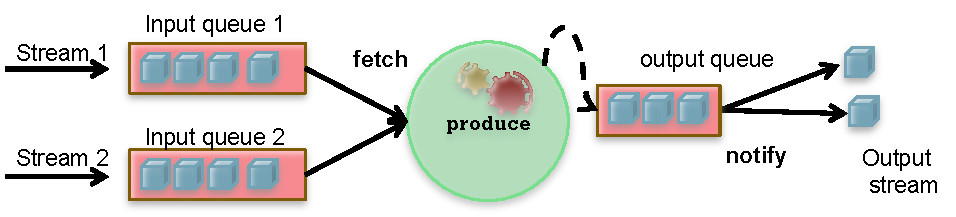
\epsfig{file = images/EPU.pdf, width = 10.5cm}}
  \caption{Event processing unit}
  \label{fig:event processing unit}
 \end{figure*}

\subsubsection{Operators}
Let $ES_i = stream(s_i), i=1,2,3 $. 
The operations applicable to event streams are defined a follows:
\paragraph{Filters.} they filter events according to their content, discarding event that do not satisfy a given predicate P. 
We note $ES_2 = Filter(ES_1, P)$. An instance e of $ES_2$ is produced if an instance $e_1$ of $ES_1$ occurs, satisfying $P(e_1) = true$.
%$\rightarrow (e \in ES_2  \rightarrow  e \in ES_1 \wedge P(e)=true)$
\paragraph{Logic Operators.} They detect the occurence of relevant event streams.
\begin{itemize}
\item \textit{Disjunction}. We note $ES_3 = OR(ES_1, ES_2)$. An instance e of $ES_3$ is produced if an instance of $ES_1$ or $ES_2$ (or both) occurs.
\item \textit{Conjunction}. We note $ES_3 = AND(ES_1, ES_2)$. An instance e of $ES_3$ is produced if an instance of both $ES_1$ and $ES_2$ occurs, regardless their order of occurrence.
\end{itemize}
\paragraph{Sequence.} This operation captures precedence orders between events from different streams. We note $ES_3= SEQ(ES_1, ES_2)$. An instance e of $ES_3$ is produced if an instance $e_1$ of $ES_1$ and $e_2$ of $ES_2$ occurs, satisfying $e_{1}.detectionTime < e_{2}.detectionTime$. 
\paragraph{Windows.} They partition a stream into finite subsets. The way each subset is constructed depend on the window specification, which can be time-based or count-based. 
\begin{itemize}
\item Time based windows define windows using time intervals:
\subitem - Fixed windows define a fixed interval [tb, te]. An event e belong to the window iff $ tb \leq e.detectionTime \leq te$
\subitem - Landmark windows define a fixed lower bound tb, such that an event e belong to the window iff $ tb \leq e.detectionTime $
\subitem - Sliding windows define a fixed duration of windows tw and the time ts after which both lower and upper bounds advance
\item Count based windows define the number of events for each window
\subitem - Fixed size windows specify a fixed size nb of each window. The input stream is partitioned in non overlapping batch, each batch containing nb events. If we consider windows of size 3, the stream $e_6, e_5,e_4, e_3, e_2, e_1$, will be partitiionned in windows [$e_6, e_5,e_4]$ and $[e_3, e_2, e_1]$
\subitem - Moving fixed size windows define a fixed number nb of events in the window, and the window is moving each time k events arrived. An event instance may be part of many windows. If we consider windows of size 3 moving after each event, the stream $e_5,e_4, e_3, e_2, e_1$ will be partitionned in windows [$e_3, e_2, e_1$], [$e_4,e_3, e_2$] and [$e_5, e_4,e_3$]
\end{itemize}

\paragraph{Aggregates.} They allows the computation of the aggregate value of an attribute over a set of event instances. They are usually combined with the use of windows to limit their scope. Aggregates operators includes max, min, count, avg and sum. 

\subsection{Architecture}
The event processing runtime is made of multiple event processing units forming an event processing network. The main components of an event processing network are the event processing units and the event channels.
\subsubsection{Event Processing Unit}
An event processing unit can be define by three types of components (see Figure \ref{fig:event processing unit}):
\begin{itemize}
\item a set of input queues, on which parts of input event streams are maintained. 
\item an operator, which implements a three step event processing logic: \textit{fetch-produce-notify}. In the first step (fetch), some events are selected from the input queues and marked as ready to be used to produce new composite events at the next step. In the second step (produce), the events selected at step 1 are used to produce new composite events according to the operator semantic. The composite events produced are stored in the output queue. In the third step (notify), the events presents in the output queue are notified either to other event processing units or to interested consumers.  
\item an output queue, which maintains events to be notified.
\end{itemize}

\subsubsection{Event Channel}
Event processing units communicate through event channels. Event channels are means of conveying event objects \cite{Luckham2011}. This can be done via standard tcp or udp connections, or a higher level communication mechanism like publish/subscribe \cite{Eugster2003} or group communication  \cite{Chockler2001} provided by a middleware layer.

\subsubsection{Deployment Architecture}
%\subsection{Architecture}
\label{sec:architecture}

The deployment architecture of our QoS based event processing system is depicted at Figure \ref{fig:architecture}.
\begin{figure}[!h]
  %\vspace{-0.2cm}
  \centering
   {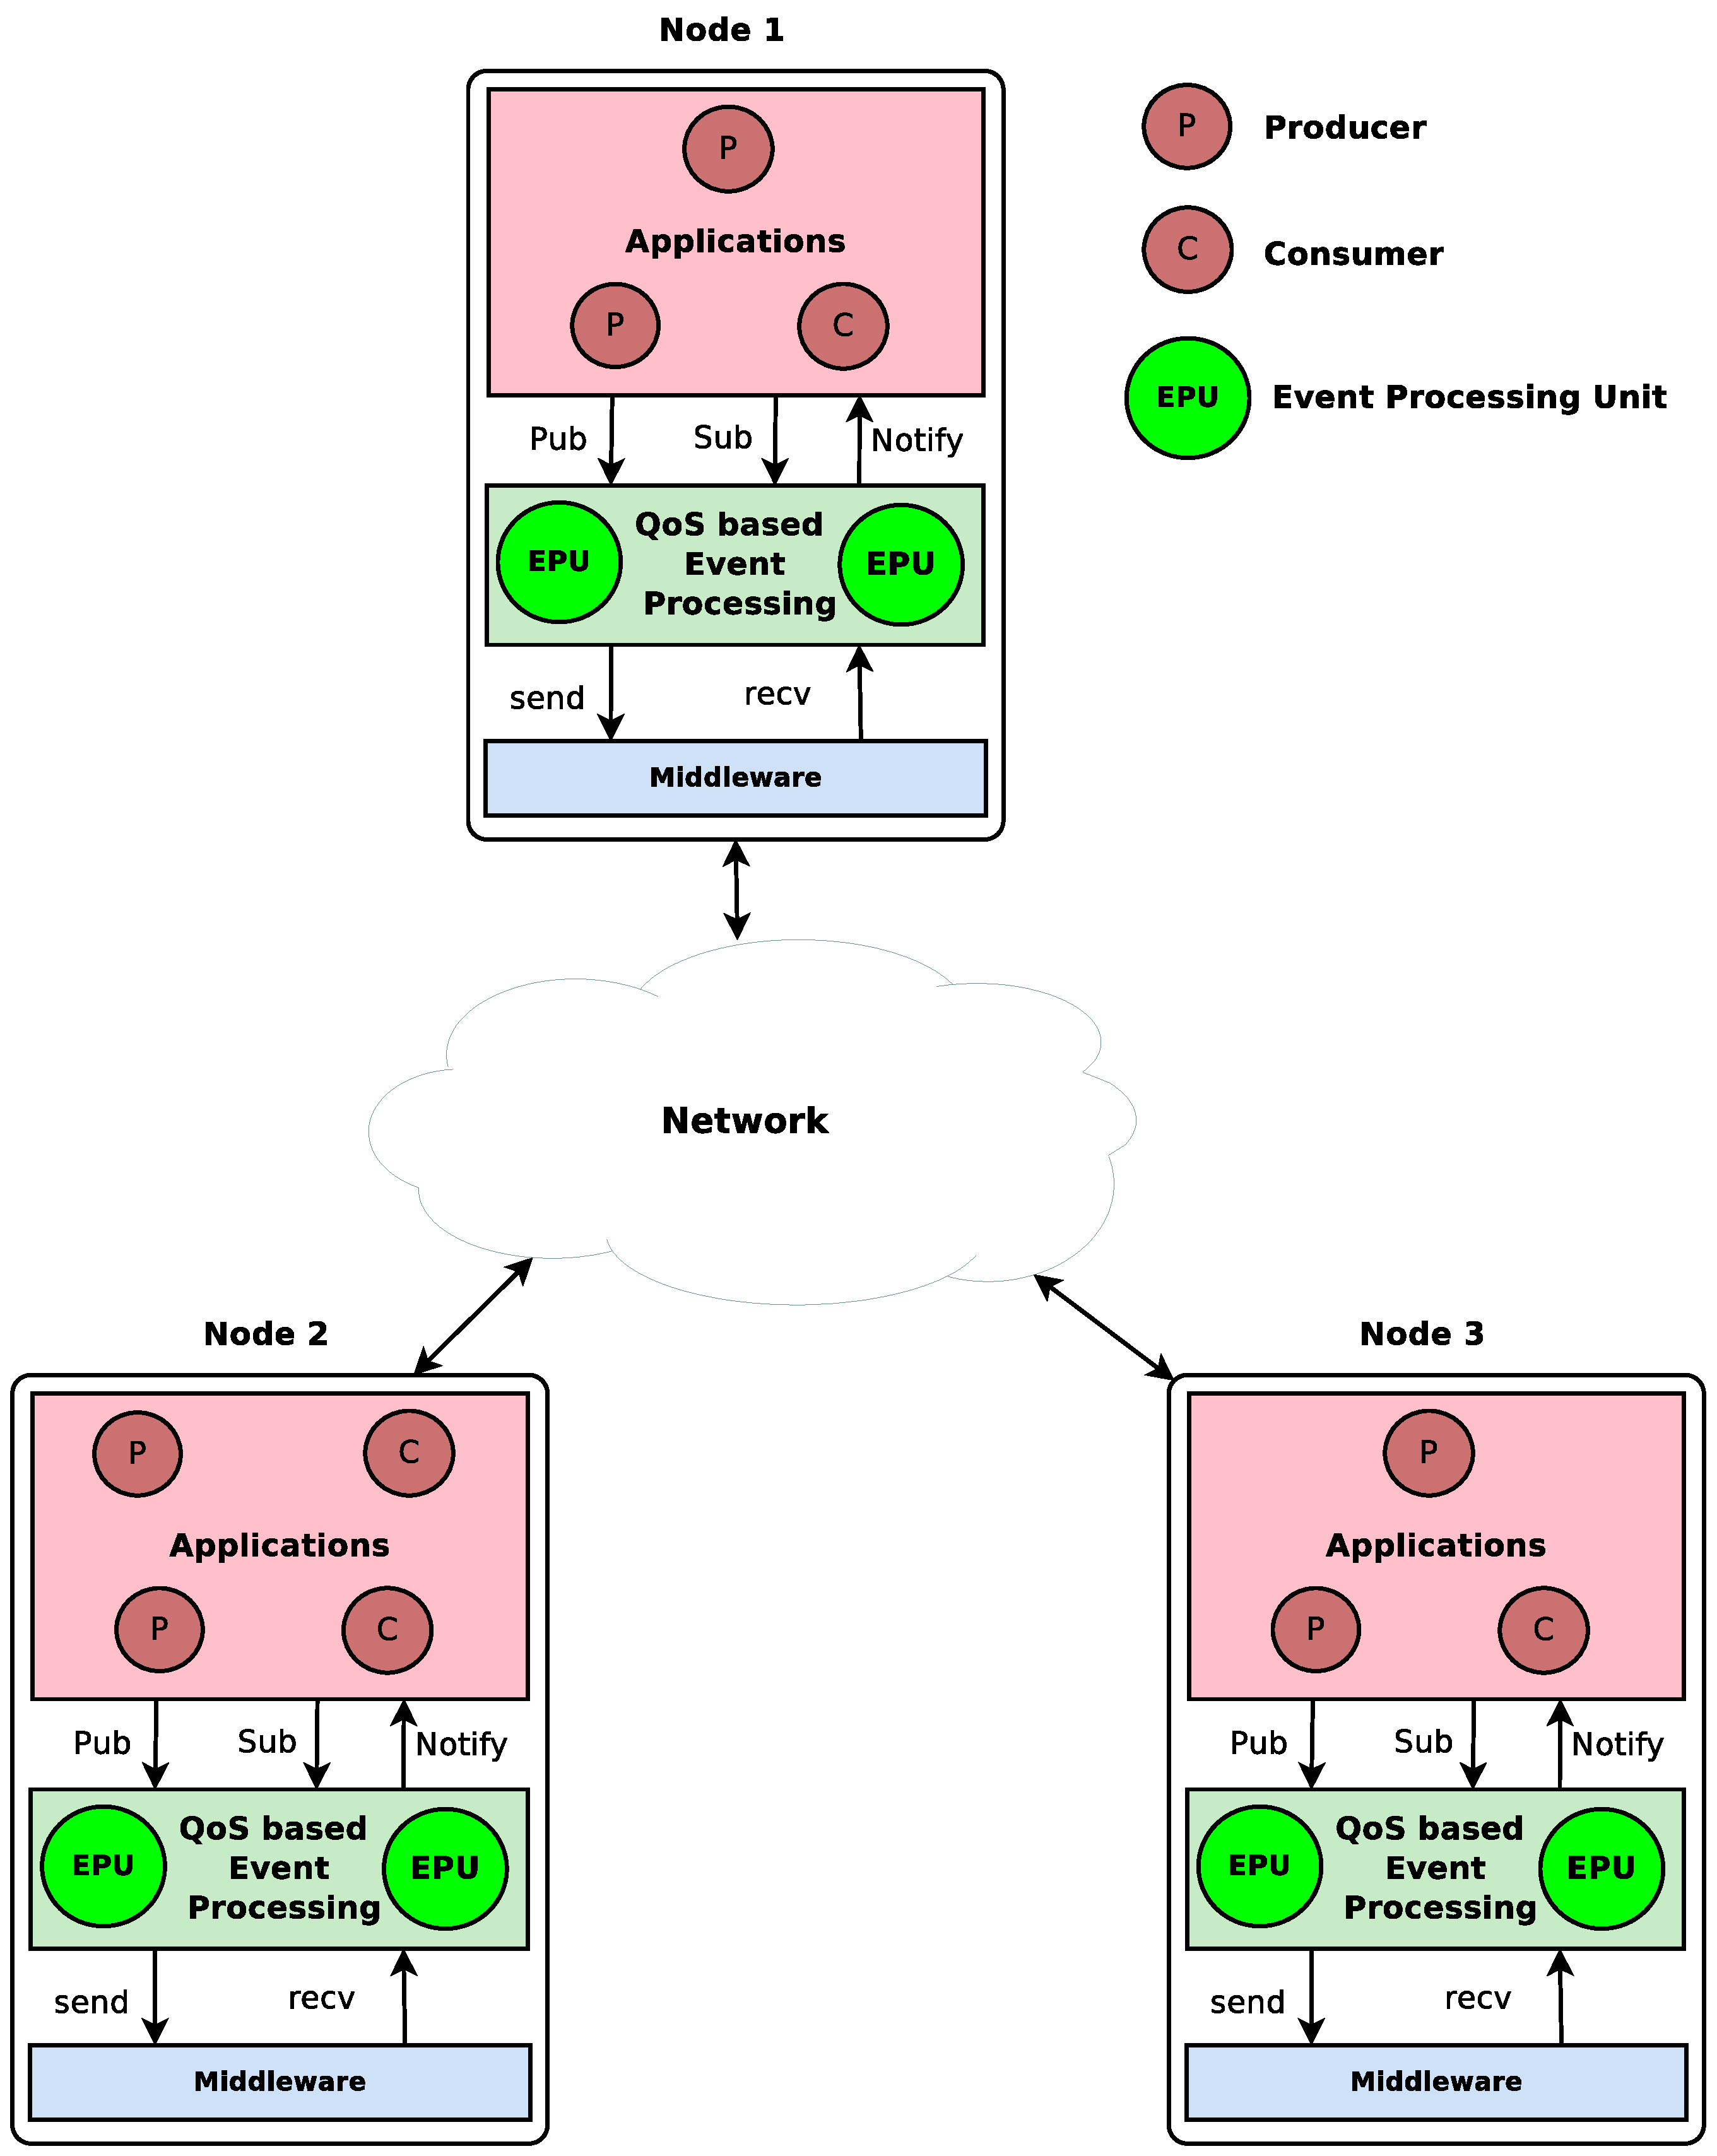
\epsfig{file = images/archi.eps, width = 7.5cm}}
  \caption{Deloyment architecture}
  \label{fig:architecture}
 \end{figure}
 The proposed framework consists of the following layers:
\begin{itemize}
\item the application layer, consisting of two types of components: event producers (sensors, smart meters, etc.), and event consumers, which subscribe to complex event patterns, with some QoS requirements.
\item the QoS based event processing layer, consisting of a set of distributed event processing units (event processing unit), implementing the event processing logic: they derive complex events from events generated by producers (simple events) or by others event processing units (complex events), as expressed in complex event subscriptions, taking into account QoS requirements. The complex events generated by an event processing unit are notified either to consumers or to other event processing units (potentially distributed) for further processing. The set of event processing units with the event channels connecting them is called the event processing network (EPN) \cite{Luckham2011}.
\item the middleware layer, providing a high-level communication mechanism (publish /subscribe or group communication) to event processing units. It relies on the underlying network layer.
\item the network layer consists of the underlying IP network providing mechanisms for transporting messages from one destination to another.  
\end{itemize}
The runtime deployment of our framework may be distributed across multiple physical networks, computers and software artifacts.
Our general vision to a QoS based complex event processing framework can be briefly described as follows: applications subscribe to composite events by issuing complex event patterns to the system, with associated QoS requirements. The system then deploys a set of distributed event processing units, which apply different strategies to meet QoS requirements. The composite events generated by the event processing units are notified to consumers. In a smart grid scenario, such an infrastructure can act as a middleware on which utility applications can rely for detecting interesting or critical situations (sensors errors, alarms, etc.) over the electrical grid, with some QoS guarantees (e.g. priority, notification latency, etc.).
\subsection{QoS Adoption in Event Processing}
\label{sec:qos_adoption} 
The QoS requirements defined by applications constrain the way event processing and notification must be achieved. To address those
QoS requirements, we identify some strategies applicable to the event processing units that allow to meet the defined QoS. Some of those strategies are correlated with properties that have to be satisfied by the middleware and/or the network layer to be really effective.

\subsubsection{Event Priority}
To model event priority, we associated to each event definition a priority attribute, which can be assigned an integer value (See Table \ref{tab:eventType}). The priority value of a simple event is defined by its producer, whereas the priority value of a composite event is computed as the maximum priority of its operand events. The higher is the priority value associate to an event instance, the higher is the event priority. Events are inserted into input and output queues according to their priority. Input and output queues are priority-based FIFO structures with limited capacity. The priority relation $\prec$ is defined as follow: \newline
$e_i \prec e_j \rightarrow$ \newline
$e_i .priority < e_{j}.priority$  $\vee$    \newline
$e_i .priority = e_{j}.priority \wedge e_i.detectionTime \leq e_j.detectionTime$ \newline
The $\prec$ relation ensure that high priority events will be notified early compared to less priority events. As consequence, the notification of a less priority event can be postponed for a significant amount of time. This issue, that we refer to as the \textit{starvation problem}, is stated more precisely as follows:
an event in the output queue may suffer the \textit{starvation problem} with respect to the notification step if after a significant number of notifications k, that event is still in the output queue, due to its priority which is less compared to that of inserted events. 

To solve the starvation problem, we associated to each event in the output queue a time to live value ttl which is initialized to an integer k. At each notification step, we decrease the ttl value of each event and nofify all the events for which the ttl value equals zero. 

For the event priority defined by applications to be really effective, there are also some assumptions that have to be made on the underlying layers of the event processing runtime. More precisely, the middleware layer must provide a FIFO delivery mechanism, allowing to convey events while preserving their notification order \cite{Chockler2001,Malekpour2011}.
\subsubsection{Memory Occupation}
Event streams received by an event processing unit are stored in the inputs queues before being processed. To process those events, the event processing unit can use some data structures. The processed events are stored in the output queue for notification. The memory occupation incurred by an event processing unit can be approximated by the memory occupation of its input queues, output queue and data structures. Whereas the maximum memory occupation of input and output queues depend on their capacities, the memory space used by data structures is operator dependent. Then, to target the memory limitation of some devices, our approach let the user specify the maximum capacity acceptable for input and output queues, and the maximum amount of memory an event processing unit can allocate for its data structure on a processing device. The management of event queues are then enrich with some strategies that decide what to do when trying to insert in a full input/output queue.

For input queue, we have two strategies which are \textit{replace and ingore }.
\begin{itemize}
\item In the replace strategy, the last event in the input queue is remove and the new event is inserted according to the $\prec$ relation;
\item In the ignore strategy, the insertion of the new event is cancelled, and the event is lost.
\end{itemize} 

For output queue, we have two strategies which are \textit{replace and notify}.
\begin{itemize}
\item In the replace strategy, the last event in the input queue is remove and the new event is inserted according to the $\prec$ relation;
\item In the notify strategy, a notification procedure is triggered before the event insertion, releasing some space for new events. 
\end{itemize} 
Sometimes, the memory footprint of an event processing unit can be dominate by the data structure used by its operator implementation. For example, an event processing unit implementing a one hour event window is more likely to consume a lot of memory, in particular in case of high input stream rate. This kind of operator dependend behaviour can be handled at the deployment phase, where high memory consuming operators are to be deployed on sites where the available memory is enough.    
\subsubsection{Network Occupation} 
As state in section \ref{sec:qos_support}, the network occupation constraint give an upper bound on the number of networked event notifications accomplished by an event processing unit per time unit. This constraint is defined on a processing site, and concerns the event processing units that are scheduled to be executed on that site. To limit the network occupation incurred by event processing units, we define the \textit{batch} notifications strategy, which consists in queuing events to be notified until they a certain size, or until a timeout has elapsed. Then, queued events are assembled and notified in batch. If the size of each group is k, this will reduce the network occupation by a factor of k. Let's assume that the limit of notifications per time unit is set to l, and the current measured value is c. If  $c > l$ , the constraint is violated. Then, applying the batch notification strategy will correct the constraint violation if the size k of each batch is choosen so that $k \geq c/l$. 

It is worth to mention that applying the batch notification strategy does not add more memory overhead, since events to be notified are maintained in the same output queue, without using an extra data structure. Thus, this strategy is not in conflict with the memory occupation constraint.
\subsubsection{Notification Latency}
The notification latency constraint imposed on an event processing unit define an upper bound on the notification latency of events produced by that event processing unit. Although desirable, it is hard to achieve a strong upper latency bound for each single event, considering the complexity of most real world networks in which EPN are deployed. In a smart grid for example, the available nerwork technologies include power line communications, wireline and wireless networks, each of them providing a different data rate \cite{Wang2011} . To target such contexts, we follow the approach of \cite{Lohrmann2013} which associate to the latency constraint definition a time span $t$, providing a concrete time frame for which the violations of the constraint can be tested . The notification latency constraint then specify an upper bound on the mean latency $\overline{nl}_{t,p}$ of events notified during the given time span t by an event processing unit p. If we call $E_t$ the events notified in a time span $t$  by event processing unit $p$, and $nl(e, s)$ the notification latency of an event $e$ generated by $p$, the notification latency constraint on $p$ define an upper bound $l$ such that:
\begin{equation}\label{eq1}
\overline{nl}_{t,p} = \frac{\sum_{e \in E_t} nl(e,p)}{|E_t|} \leq l
\end{equation} 
The notification latency of an event can be derived by its production time (\textit{productionTime} attribute) and its reception time (\textit{receptionTime} attribute) by the following formula:
\begin{equation}\label{eq2}
nl(e,p) = e._{receptionTime} - e._{productionTime}
\end{equation} 
If $\overline{nl}_{t,p} > l$, we have a latency constraint violation. This can be due to two factors:
\begin{itemize}
\item The time spend in the event processing unit output queue, which depend on the size of the ouput queue.
\item The network path between the event producer and the consumer, characterized by the number of hops and the speed of network links.
\end{itemize}
To fix a latency constraint violation, our strategy is to adjust the size of an event processing unit output queue, in order to reduce the time an event has to wait before being sent over the network. The intuition is that if the observed mean latency $\overline{nl}_{t,p}$ is lower than the maximum latency $l$ by a factor $r = \frac{\overline{nl}_{t,p}}{l}$, then we will reduce the size of the ouput queue by a factor r. Then, in case the latency constraint is violate for an event processing unit, we adjust its output queue size from its old value $k$ to the new value $k^*$ such that
\begin{equation}\label{eq3} 
 k^* = max(1,\lfloor \frac{k}{r} \rfloor) = max(1, \lfloor \frac{k \times{l}}{\overline{nl}_{t,p}} \rfloor)
 \end{equation}
\section{\uppercase{Implementation}}
\label{sec:implem}
To do...


\section{\uppercase{Conclusion}}
\label{sec:conclusion}
The monitoring of large scale distributed systems like smart grids, telecommunications can be done using an event based approach, where events generated by distributed sources are processed by distributed  event processing units and notified to interested consumers. Since the invocation of business critical processes is now triggered by events, the QoS of the event processing infrastructure becomes a key aspects. In this paper, we have identified key QoS dimensions applicable to distributed systems like smart grids, and presented our approach for a QoS based event processing. It is worth to mention that most of our proposed system still at an early stage and we still need a long research to accomplish a “complete” system that fully applies QoS based event processing in distributed environments. 

\bibliographystyle{apalike}
{\small
\bibliography{example}}

\vfill
\end{document}